\documentclass[t, pdftex]{beamer}  
%Use Cockrell School Theme.  Optional department name.  Must %ecape, i.e. use 
%backslash, to preserve spaces.  The default is ``Cockrell School of Engineering''
\usetheme[]{Cockrell}                 
%\usetheme[dept=Aerospace\ Engineering\ and\ Engineering\ Mechanics]{cockrell}                 
%\usetheme[dept=Biomedical\ Engineering]{cockrell}                 
%\usetheme[dept=Chemical\ Engineering]{cockrell}                 
%\usetheme[dept=Civil,\ Architectural\ and\ Environmental\ Engineering]{cockrell}                 
%\usetheme[dept=Electrical\ and\ Computer\ Engineering]{cockrell}                 
%\usetheme[dept=Mechanical\ Engineering]{cockrell}                 
%\usetheme[dept=Materials\ Science\ and\ Engineering]{cockrell}                 
%\usetheme[dept=Petroleum\ and\ Geosystems\ Engineering]{cockrell}                 

% Add preamble packages here
%\usepackage{etex}
%\usepackage[bigfiles]{media9}
%\graphicspath{{./figs/}}
\usepackage{bussproofs}
\usepackage[export]{adjustbox}
%Enable cancelto in math
\usepackage{cancel}
\renewcommand{\CancelColor}{\color{utorange}}

%Add bibliography file location for citiation
\bibliography{example.bib}


\title{Presenting finite posets \\(with monotone maps?)}
\subtitle{... using string diagrams}
\author{Sam Balco}
% \institute{Special Event}
\date{\today}


\newenvironment{bprooftree}
  {\leavevmode\hbox\bgroup}
  {\DisplayProof\egroup}


\begin{document}

%Creates title frame from title, subtitle, author, institute, and date above
\titleframe

%Supports table of contents
\frame{\frametitle{Outline}\tableofcontents}

%Section commands will define what's shown in TOC
\section{What are string diagrams?}

%First frame
\begin{frame}
    \frametitle{What are string diagrams?}
    They are a bit like legos!
    \begin{center}
        
\includegraphics{figures/lego.pdf}
    \end{center}
\end{frame}

\begin{frame}
    \frametitle{What are string diagrams?}
    We can combine legos/string diagrams in two different ways:
    \begin{center}
        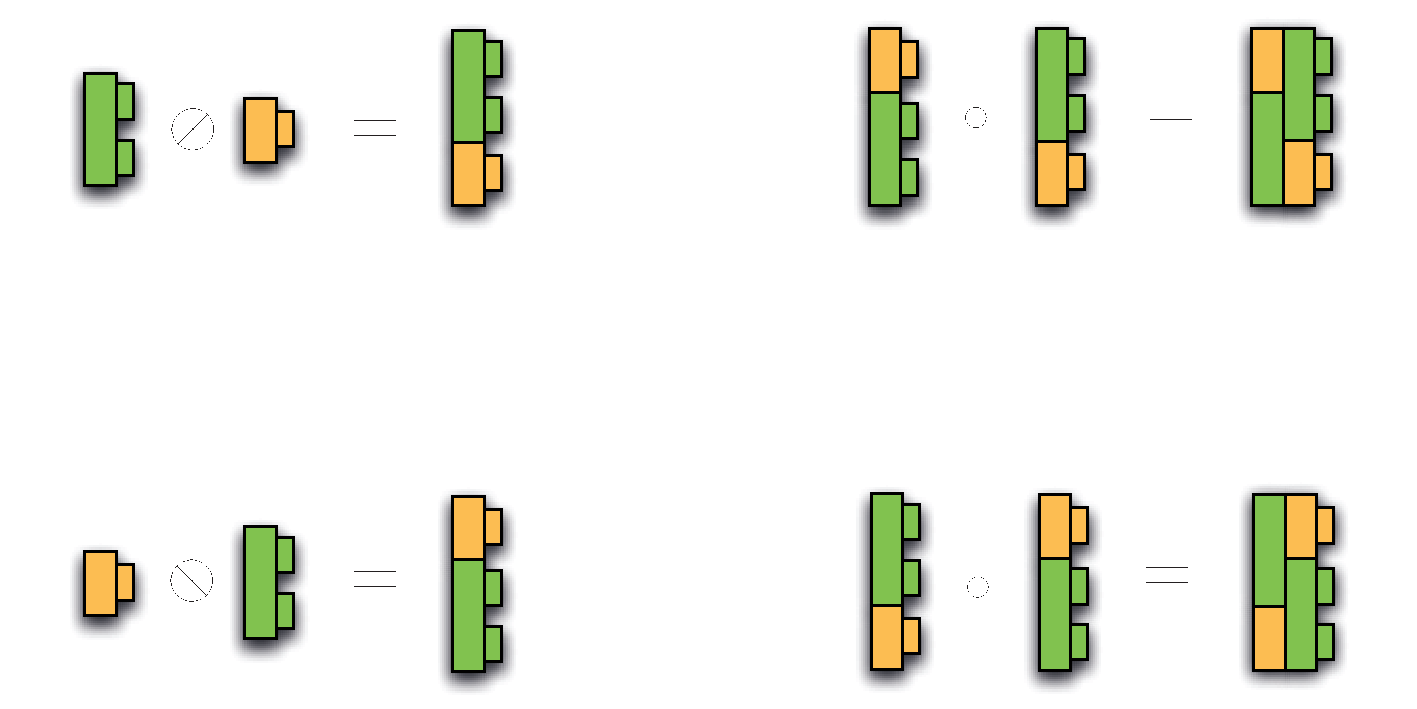
\includegraphics[width=\textwidth,keepaspectratio]{figures/lego2.pdf}
    \end{center}
\end{frame}

\begin{frame}
    \frametitle{What are string diagrams?}
    We can combine legos/string diagrams in two different ways:
    \begin{center}
        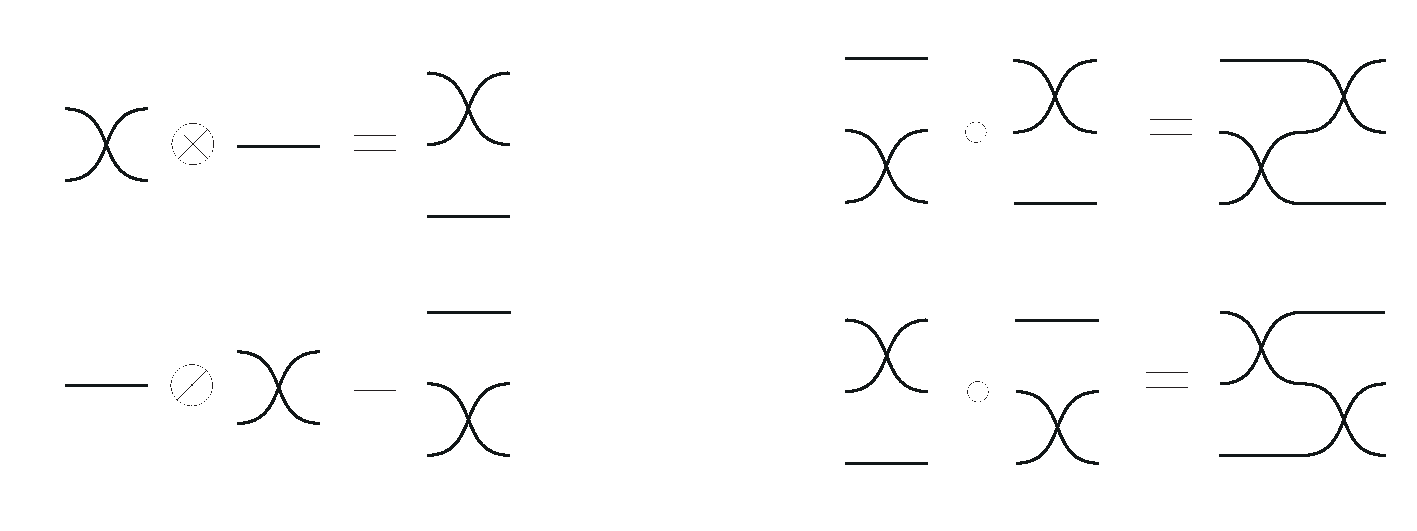
\includegraphics[width=\textwidth,keepaspectratio]{figures/lego3.pdf}
    \end{center}
\end{frame}

\section{String diagrams algebraically}

\begin{frame}
    \frametitle{String diagrams algebraically}
    We can assign each string a type, given by the number of input ports (on the left) and the number of output ports on the right:
    \begin{table}[]
        \centering
        \begin{tabular}{rrrr}
            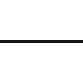
\includegraphics[valign=m, width=1cm]{figures/string2.pdf} $\ : (1,1)$ & 
            
\includegraphics[valign=m, width=1cm]{figures/string1.pdf} $\ : (2,2)$ & 
            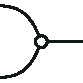
\includegraphics[valign=m, width=1cm]{figures/string4.pdf} $\ : (2,1)$ &
            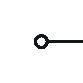
\includegraphics[valign=m, width=1cm]{figures/string3.pdf} $\ : (0,1)$\\
            % \hrulefill & \hrulefill & \hrulefill & \hrulefill \\
            & & & \\
            $id : (1,1)$ & 
            $\gamma : (2,2)$ & 
            $\mu \ : (2,1)$ & 
            $\eta \ : (0,1)$
        \end{tabular}
    \end{table}
    \par
    % \begin{table}[]
    %     \centering
    %     \begin{tabular}{lll}
            
    %     \end{tabular}
    % \end{table}
    % \par
    \begin{table}[]
        \centering
        \begin{tabular}{ll}
            \begin{bprooftree}
                \AxiomC{$S:(k,l)$}
                \AxiomC{$T:(m,n)$}
                \BinaryInfC{$S \otimes T:(k + m,l + n)$}
            \end{bprooftree} &
            \begin{bprooftree}
                \AxiomC{$S:(k,l)$}
                \AxiomC{$T:(l,m)$}
                \BinaryInfC{$S \circ T:(k,m)$}
            \end{bprooftree}
        \end{tabular}
    \end{table}
\end{frame}

\begin{frame}
    \frametitle{String diagrams algebraically}
    \begin {center}
        $\Bigg(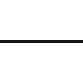
\includegraphics[valign=m, width=1cm]{figures/string2.pdf} \otimes
        
\includegraphics[valign=m, width=1cm]{figures/string1.pdf} \Bigg) \circ 
        \Bigg(
\includegraphics[valign=m, width=1cm]{figures/string1.pdf} \otimes
        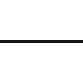
\includegraphics[valign=m, width=1cm]{figures/string2.pdf} \Bigg)$\\
        \vspace{.5cm}
        $=$\\
        \vspace{.5cm}
        $(id \otimes \gamma) \circ (\gamma \otimes id)$\\
        \vspace{.5cm}
        $=$\\
        \vspace{.5cm}
        $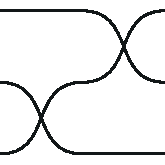
\includegraphics[valign=m, width=2cm]{figures/dia1.pdf}$\\
        
        
    \end{center}
\end{frame}

\section{Presenting finite sets and functions}
\begin{frame}
    \frametitle{Presenting finite sets and functions}
    So what can we do with $id, \gamma, \mu$ and $\eta$?
    \par \ 
    \par
    Say we have function $f : [5] \to [5]$ (where $[n] = \{0\hdots n-1\}$):
    \begin{align*}
        f(0) &= 1\\
        f(1) &= 0\\
        f(2) &= 4\\
        f(3) &= 3\\
        f(4) &= 1
    \end{align*}

\end{frame}

\begin{frame}
    \frametitle{Presenting finite sets and functions}
    So what can we do with $id, \gamma, \mu$ and $\eta$?
    \par \ 
    \par
    We can express this function as a string diagram:
    \begin{center}
        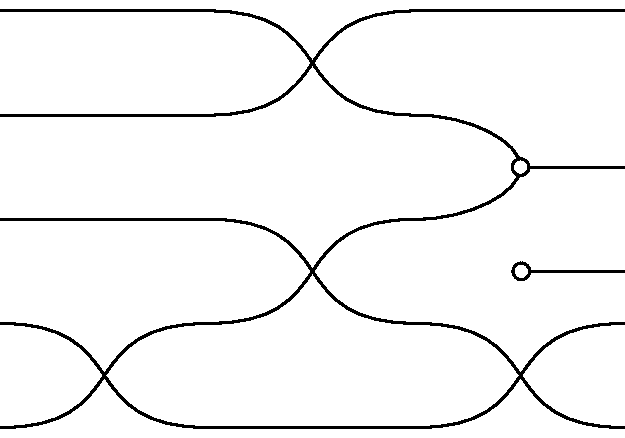
\includegraphics[height=4.5cm,keepaspectratio]{figures/dia2.pdf}
    \end{center}

\end{frame}


\begin{frame}
    \frametitle{Presenting finite sets and functions}
    So what can we do with $id, \gamma, \mu$ and $\eta$?
    \par \ 
    \par
    Or alternatively:
    \begin{center}
        $(id \otimes id \otimes id \otimes \gamma)\ \circ$\\
        $(\gamma \otimes \gamma \otimes id)\ \circ$\\
        $(id \otimes \mu \otimes \eta \otimes \gamma)$
    \end{center}

\end{frame}

\begin{frame}
    \frametitle{Presenting finite sets and functions}
    
    \begin{center}
        What happens if we remove $\gamma$ from our list of possible generators?
    \end{center}

\end{frame}


\section{Refresher on posets}

\begin{frame}
    \frametitle{Refresher on posets}
    A \textit{poset} is a set $S$, together with a partial order relation $\leq_S\ : S \times S$, which is \textit{reflexive}, \textit{transitive} and \textit{antisymmetric}.

    For example, for $S = \{a,b,c,d,e\}$ and $a \leq_S c ,\allowbreak a \leq_S d,\allowbreak b \leq_S d,\allowbreak c \leq_S e,\allowbreak d \leq_S e$, we can draw the following diagram, representing the poset:
    \begin{center}
    \begin{tikzpicture}
    \node (a) at (0,0) {$a$};
    \node (c) at (-1,1) {$c$};
    \node (d) at (1,1) {$d$};
    \node (e) at (0,2) {$e$};
    \node (b) at (2,0) {$b$};
    \node (f) at (2,2) {$f$};
    \draw (a) -- (c);
    \draw (a) -- (d);
    \draw (b) -- (d);
    \draw (c) -- (e);
    \draw (d) -- (e);
    \draw (d) -- (f);
    \end{tikzpicture}
    \end{center}
\end{frame}

\begin{frame}
    \frametitle{Refresher on posets}
    \begin{center}
    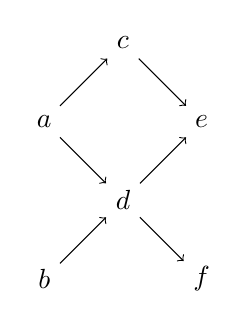
\begin{tikzpicture}
    \node (a) at (0,0) {$a$};
    \node (b) at (0,-2) {$b$};
    \node (c) at (1,1) {$c$};
    \node (d) at (1,-1) {$d$};
    \node (e) at (2,0) {$e$};
    \node (f) at (2, -2) {$f$};
    \draw[->] (a) -- (c);
    \draw[->] (a) -- (d);
    \draw[->] (b) -- (d);
    \draw[->] (c) -- (e);
    \draw[->] (d) -- (e);
    \draw[->] (d) -- (f);
    \end{tikzpicture}
    \end{center}
\end{frame}

\section{Presenting posets}

\begin{frame}
    \frametitle{Presenting posets}
    \begin{center}
    \begin{tikzpicture}
    \node (a) at (0,0) {$\circ$};
    \node (b) at (0,-2) {$\circ$};
    \node (c) at (1,1) {$\circ$};
    \node (d) at (1,-1) {$\circ$};
    \node (e) at (2,0) {$\circ$};
    \node (f) at (2, -2) {$\circ$};
    \draw[->] (a) -- (c);
    \draw[->] (a) -- (d);
    \draw[->] (b) -- (d);
    \draw[->] (c) -- (e);
    \draw[->] (d) -- (e);
    \draw[->] (d) -- (f);
    \end{tikzpicture}
    \end{center}
\end{frame}

\begin{frame}
    \frametitle{Presenting posets}
    \begin{center}
    \begin{tikzpicture}
    \node (a) at (0,0) {$\circ$};
    \node (b) at (0,-2) {$\circ$};
    \node (c) at (1,1) {$\bullet$};
    \node (d) at (1,-1) {$\bullet$};
    \node (e) at (2,0) {$\circ$};
    \node (f) at (2, -2) {$\circ$};
    \draw[->] (a) -- (c);
    \draw[->] (a) -- (d);
    \draw[->] (b) -- (d);
    \draw[->] (c) -- (e);
    \draw[->] (d) -- (e);
    \draw[->] (d) -- (f);
    \end{tikzpicture}
    \end{center}
\end{frame}

\begin{frame}
    \frametitle{Presenting posets}
    \begin{center}
        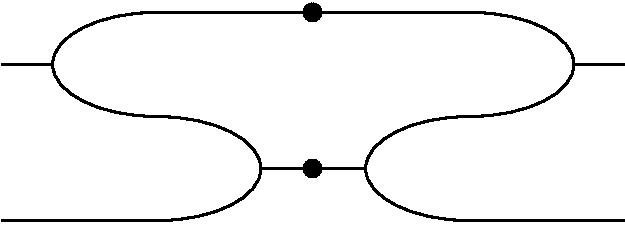
\includegraphics{figures/dia3.pdf}
    \end{center}
\end{frame}


\lastframe%
\end{document}
